\chapter{Технологический раздел}
\label{cha:impl}

Для реализации программного продукта необходимо выбрать язык программирования, среду разработки, а также библиотеки, которые позволят сделать приложение функциональным и гибким по отношению к возможным будущим изменениям, модификации, расширению функционала.
В данном разделе приводится краткое описание выбранных средств, а также требования для функционирования программного обеспечения и описание его архитектуры.

\section{Выбор средств и инструментов разработки}
\subsection{Выбор языка программирования}
В качестве языка программирования для реализации программного обеспечения был выбран язык Python. Это высокоуровневый язык программирования общего назначения, поддерживающий различные парадигмы программирования, а также портированный почти на все известные платформы. Синтаксис ядра Python минималистичен, при этом стандартная библиотека включает большой объем полезных функций. Также Python имеет богатую документацию с большим количеством примеров. % возможно ссылка
Описанные особенности положительно влияют на скорость разработки программного обеспечения.

В данной работе выбор языка Python обусловлен следующими причинами:
\begin{itemize}
	\item богатый выбор различных библиотек, в том числе и библиотек, используемых для решения задач машинного обучения;
	\item наличие подробной документации с примерами;
	\item наличие опыта разработки приложений на данном языке;
	\item большое количество проектов с открытым исходным кодом в области задач машинного обучения.
\end{itemize}

\subsection{Выбор среды разработки}
В качестве среды разработки был выбран текстовый редактор Visual Studio Code. Данный выбор обусловлен следующими причинами:

\begin{itemize}
	\item Данный текстовый редактор поддерживается большинством платформ;
	\item Является более "легковесным" по сравнению с полноценными интегрированными средами разработки, такими как PyCharm, Eclipse, Visual Studio;
	\item Имеется возможность установки дополнительных плагинов для разработки на определенном языке, в том числе и для разработки на языке Python;
	\item Интеграция с системой контроля версий Git.
\end{itemize} 

\subsection{Выбор базы данных}
Так как в данной работе применяются алгоритмы машинного обучения, то встает вопрос хранения данных, используемых для обучения классификатора.
В качестве базы данных была выбрана реляционная база данных SQLite. Выбор именно этой базы данных обусловлен рядом следующих причин:

\begin{itemize}
	\item кросс-платформенность;
	\item отсутствие необходимости настройки сервера СУБД, так как все данные и параметры настроек базы данных хранятся в одном единственном файле;
	\item высокая производительность;
	\item небольшой объем занимаемой памяти;
	\item возможность использования многих языков программирования, в том числе и Python.
\end{itemize}

\subsection{Система контроля версий}
В процессе разработки программного обеспечения использовалась система контроля версий Git. Система контроля версий позволяет вносить в проект атомарные изменения, направленные на решения каких-либо задач. В случае обнаружения ошибок или изменения требований, внесенные изменения можно отменить. Кроме того, с помощью системы контроля версий решается вопрос резервного копирования.

Выбор системы контроля версий Git обусловлен следующими ее особенностями:

\begin{itemize}
	\item Данная система контроля версий является децентрализованной, что позволяет иметь несколько независимых резервных копий проекта;
	\item Поддерживается хостингом репозиториев GitHub;
	\item Предоставляет широкие возможности для управления изменениями проекта и просмотра истории изменений.
\end{itemize}


\section{Описание используемых библиотек}

Как было сказано ранее, существует множество библиотек, написанных для языка python, которые позволяют решать множество самых разнообразных задач. В связи с этим следует привести описание основных библиотек, используемых при разработке данного программного обеспечения.

\subsection{Библиотека для работы с базами данных}
В качестве библиотеки для работы с базой данных была выбрана библиотека peewee. Данная библиотека является достаточно легковесной и легко устанавливается с помощтю пакетного менеджера pip. Также она реализована с поддержкой технологии ORM(англ. Object-Relational Mapping), % возможно,ссылка
что обеспечивает работу с данными в терминах классов языка программирования, а не в терминах таблиц данных базы SQLite.

\subsection{Библиотека для графического интерфейса}
Для написания части приложения, отвечающего за взаимодействие с пользователем, была выбрана библиотека кросс-платформенная библиотека tkinter. Данная библиотека 
позволяет создавать приложения с использованием различных графических компонентов. Также следует заметить, что данная библиотека содержится в стандартной библиотеке языка Python, что безусловно является преимуществом, так как не требуется дополнительная её установка. Еще одним преимуществом данной библиотеки является хорошая документация с большим количеством примеров.

\subsection{Библиотека для машинного обучения}
В связи с ростом популярности технологий машинного обучения для различных языков программирования было разработано множество библиотек, тем или иным образом связанных с темой машинного обучения.К наиболее популярным библиотекам, поддерживаемыми языком Python, можно отнести Scikit-Learn, Theano, TensorFlow, Keras.

В данной работы для решения задачи классификации была выбрана библиотека Scikit-Learn. Данная библиотека предоставляет следующие возможности для решения задач классификации:

\begin{itemize}
	\item Готовая реализация множества алгоритмов классификации: алгоритм опорных векторов, алгоритм k-ближайших соседей, алгоритм наивной байесовской классификации и др.;
	\item Удобный доступ к необходимым компонентам;
	\item Перекрестная проверка (Cross Validation): для оценки эффективности работы модели на независимых данных;
	\item Оптимизация параметров алгоритма (Parameter Tuning): для получения максимально эффективной отдачи от модели;
	\item Встроенные алгоритмы нормализации данных, для более эффективного обучения модели.
\end{itemize}

\newpage
\section{Описание классов}
При разработке ПО использовался преимущественно объектно-ориентированный подход. Отношения основных классов, используемых в программе, представлены на диаграмме классов(рисунок \ref{impl:diagramm}).

\begin{figure}[h!]
	\centering
	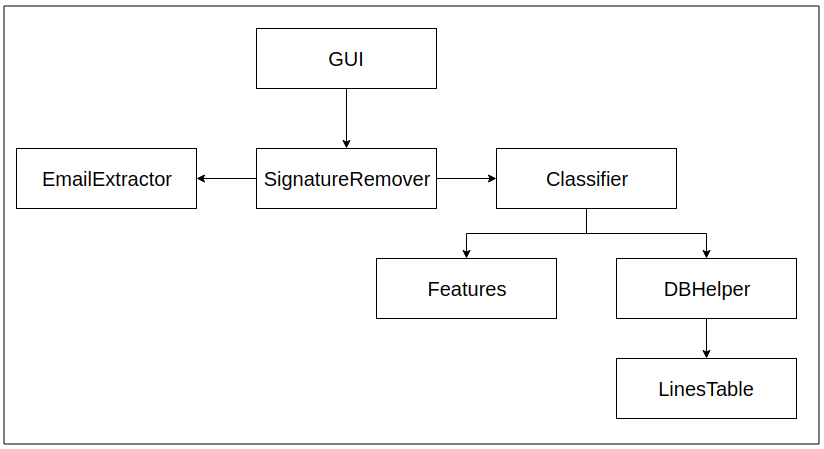
\includegraphics[width=\textwidth]{inc/img/diagramm.png}
	\caption{Диаграмма классов}
	\label{impl:diagramm}
\end{figure}


Класс \textbf{LinesTable} описывает таблицу в базе данных, которая содержит данные для обучения классификатора. Данный класс является наследником класса Model библиотеки peewee.

Класс \textbf{DBHelper} предоставляет набор методов для работы с базой данных: создание таблицы, загрузка и выгрузка данных для обучения.

Класс \textbf{Classifier} описывает методы для обучения классификатора, его сохранения в файл, а также ряд методов для классификации строк электронного письма на основе ранее обученного классификатора.

Класс \textbf{Features} описывает функционал для предварительной обработки исходных данных с целью приведения их к виду вектора признаков.

Класс \textbf{EmailExtractor} отвечает за получение текста электронного письма из почтового ящика пользователя.

Класс \textbf{GUI} является контроллером, который отвечает за пользовательский ввод и отображение информации, а так же инициализирует работу алгоритма удаления подписи.

Класс \textbf{SignatureRemover} отвечает за решение задачи удаления подписи из текста электронного письма на основе данных, полученных от пользователя, используя методы классов EmailExtractor и Classifier. Полученный результат передается классу GUI с целью выдачи результата пользователю.

\section{Требования к системе пользователя}

Разработанное программное обеспечение состоит из двух приложений: консольное приложение для загрузки исходных данных в базу данных и обучения классификатора, графическое приложение для демонстрации работы метода удаления подписи из текстов электронных писем.
Стоит заметить, что для конечного пользователя интерес представляет только графическое приложение, которое использует файл с обученным классификатором, полученный в результате работы консольного приложения, используемого непосредственно разработчиком.

Разработанное графическое приложение способно запускаться на широком круге систем, их технические характеристики не имеют принципиального значения.  К основным требованиям, необходимым для корректной работы приложения, относятся:
\begin{itemize}
	\item Предустановленный интерпретатор Python 3.6 или более поздний;
	\item Файлы библиотек scikit-learn, numpy, scipy;
	\item Подключение к сети Интернет;
	\item Наличие у пользователя почтового ящика gmail.
\end{itemize}

Стоит заметить, что большинство библиотек, используемых приложением(email, imaplib, tkinter) не требуют дополнительной установки, так как являются частью стандартной библиотеки, устанавливаемой вместе с интерпретатором Python.

\section{Тестирование ПО}

Так как результат удаления подписи из текста электронного письма зависит от работы классификатора, то необходимо протестировать корректность функций, влияющих на его обучение.
К таким функциям прежде всего следует отнести функции, представляющие строки письма в виде вектора признаков. 
Некорректное выделение признаков отрицательно скажется на обучении классификатора, что в дальнейшем может привести к снижению качества классификации строк письма. В связи с этим было проведено модульное тестирование функций, отвечающих за выделение признаков.

Для тестирования и оценки параметров обученной модели классификатора имеющаяся выборка была разделена на две части, одна из которых использовалась непосредственно для обучения, а другая - для тестирования полученной модели и ее оценки с использованием параметров, описанных в пункте 1.5.3.

\section{Описание пользовательского приложения}
Разработанное приложение представляет из себя окно, содержащее поля для ввода пользовательских данных (адрес почты, пароль, номер письма), поля для отображения исходного текста письма и текста письма после удаления подписи, а также кнопки "Помощь" и "Удалить подпись". 
Интерфейс пользовательского приложения представлен на рисунке \ref{impl:interface}. 

\begin{figure}[h!]
	\centering
	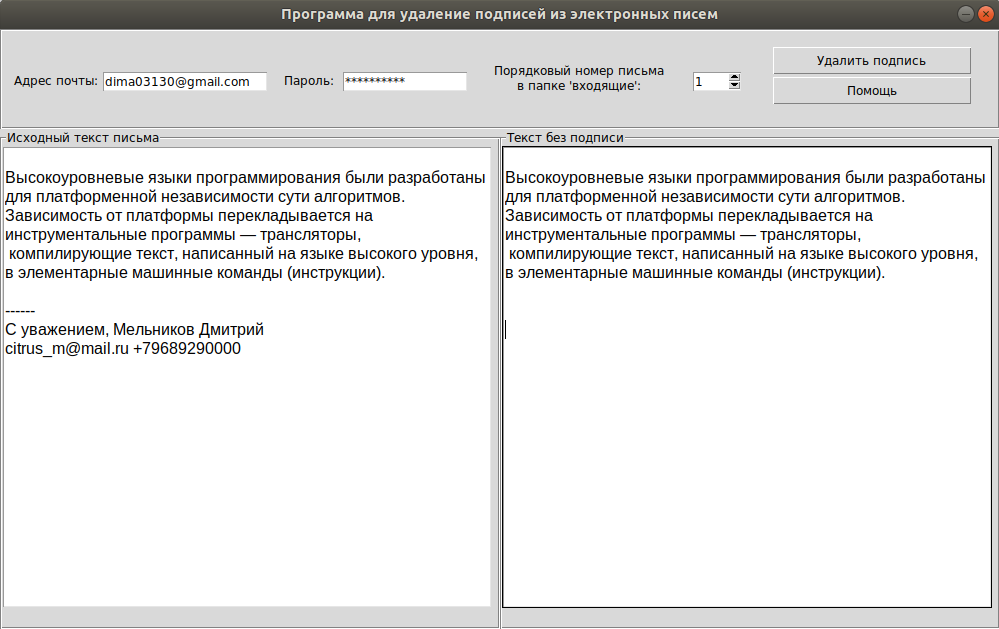
\includegraphics[width=\textwidth]{inc/img/interface.png}
	\caption{Интерфейс пользовательского приложения}
	\label{impl:interface}
\end{figure}

Приложение предоставляет пользователю две функции: удаление подписи и вывод информации о приложении. Для того, чтобы получить информацию о приложении, пользователь должен нажать на кнопку "Помощь". Для удаления подписи из письма пользователю следует ввести адрес электронной почты, пароль и порядковый номер письма в папке "входящие"  почтового ящика, а затем нажать кнопку "Удалить подпись". В случае успешной загрузки электронного письма в соответствующих полях отобразятся исходный текст письма и текст без строк, которые были классифицированы как строки, относящиеся к подписи. Также пользователь получить уведомление о том, сколько строк было удалено из текста письма.

В ходе работы программы возможно следующие ошибки и исключительные ситуации, возникающие в результате некорректных действий пользователя или по причинам, не зависящим от действий пользователя:

\begin{itemize}
	\item Введены некорректные данные учетной записи gmail;
	\item Указан порядковый номер письма, превышающий общее количество писем;
	\item Нестабильное интернет соединение;
	\item Тело электронного письма представлено не в виде текста.
\end{itemize}

Все из описанных ситуаций обрабатываются программой и выдаются в виде сообщений пользователю (рисунок \ref{impl:errors}).

\newpage
\begin{figure}[h!]
	\centering
	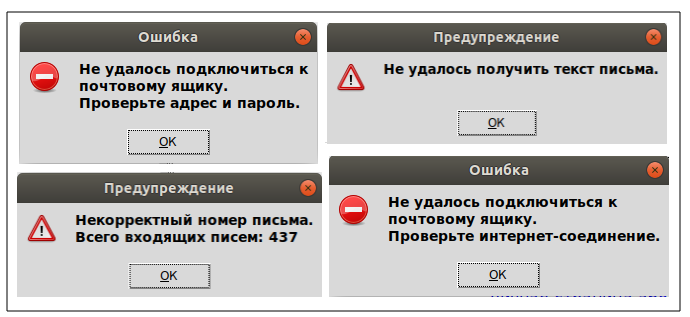
\includegraphics[width=\textwidth]{inc/img/errors.png}
	\caption{Ошибки и исключительные ситуации}
	\label{impl:errors}
\end{figure}


\newpage
\section{Выводы}
В технологическом разделе проведен анализ существующих средств разработки программного обеспечения и описан выбор средств для решения поставленной задачи. Также обоснован выбор языка программирования, среды разработки и системы контроля версий в соответствии с задачами, которые стоят перед программным комплексом, и приведено краткое описание используемых библиотек. Описаны основные классы программы, а также интерфейс разработанного приложения.

%%% Local Variables:
%%% mode: latex
%%% TeX-master: "rpz"
%%% End:
